\documentclass[times, utf8, seminar, numeric]{fer}
\usepackage{booktabs}
 \usepackage{url}
\usepackage{graphicx}
\usepackage{float}
\begin{document}

% Ukljuci literaturu u seminar
\nocite{*}

% TODO: Navedite naslov rada.
\title{Vlastita implementacija filtera: \protect\\ The Logarithmic Dynamic Cuckoo Filter}

% TODO: Navedite vaše ime i prezime.
\author{Fran Ostroški, Elena Wachtler}

% TODO: Navedite ime i prezime voditelja.
\voditelj{Mirjana Domazet-Lošo}

\maketitle

\tableofcontents

\chapter{Uvod}

TODO: Spomenuti sve izvore iz literature, točno što je koji od njih napravio i kako se jedan razlikuje od drugog (ovo se boduje, čak 3 boda, baš se moraju spomenuti izvori u tekstu, tako piše u uputama). \\

Ovaj seminar opis je projekta u sklopu kolegija Bioinformatika 1 Fakulteta elektrotehnike i računarstva Sveučilišta u Zagrebu, a predstavlja vlastitu implementaciju takozvanog cuckoo filtera, točnije njegovu dinamičku logaritamsku varijantu. \\

Cuckoo filter probabilistička je struktura podataka koja se koristi za određivanje pripadnosti zadanog elementa nekome skupu. Sam filter nastao je kao proširenje već postojećih Bloom filtera, a naziv je dobio prema ptici kukavici koja izbacuje jaja iz tuđih gnijezda kako bi ubacila svoja. Iako je riječ o općenitim podatcima, cuckoo filter često se primjenjuje u bioinformatici jer je pogodan za određivanje pripadnosti podnizova nukleotidnih slijedova nekom većem nizu nukleotida ili provjeru nalaze li se podnizovi jednog slijeda u nekom drugom slijedu.

Pripadnost elementa nekom skupu ovom strukturom ne možemo garantirati, jer zbog implementacije algoritma postoji malena vjerojatnost za lažno pozitivne (eng. \textit{false positive}) i lažno negativne (eng. \textit{false negative}) rezultate. Upravo zbog toga što postoji određena vjerojatnost pogreške, cuckoo filter je probabilistički. Međutim, nepripadnost nekom skupu može se pouzdano odrediti. \\

TODO NAPOMENA: u bibtex fileu nedostaje jedan izvor, nisam mogla naći njegov .bib: 
Fan et al. 2013. Cuckoo Filter: Better Than Bloom; https://www.cs.cmu.edu/~binfan/papers/login cuckoofilter.pdf - našla sam samo za Practically Better Than Bloom.

\chapter{Opis algoritma}
TODO Mogu se i ovdje koristiti izvori, možda čak i bolje nego da se koriste u Uvodu, iako se mogu i u uvodu spomenuti.

\begin{flushleft}
\textbf{Vizualizacija algoritma na jednostavnom primjeru}
\end{flushleft}


U općenitom slučaju, cuckoo filter sastoji se od nizova memorijskih lokacija koje se nazivaju \textit{bucketima}. Bucketi mogu imati mjesta za više unosa, ali u ovom jednostavnom primjeru svaki bucket moći će primiti  po jedan uneseni podatak.

Neka je dan jedan kratak nukleotidni slijed, npr. AACTGAT, te se kao ulazi u filter trebaju unijeti svi njegovi k-meri, za k = 3. To su : AAC, ACT, CTG, TGA i GAT . \\
U prvom koraku algoritma za svaki unos računaju se dva sažetka (eng. \textit{hash}) pomoću odabranih funkcija sažimanja (tzv. hash funkcija).

\begin{figure}[H]
  \centering
  \setlength{\intextsep}{5pt}
  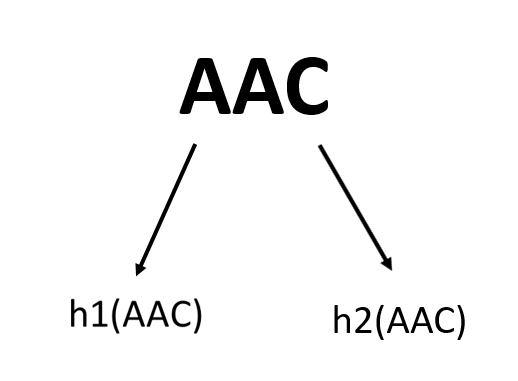
\includegraphics[scale = 0.75]{images/hashing.png}
  \caption{Generiranje hasha - Fran Ostroški}
  \label{fig_hash}
\end{figure}

U drugom se koraku iz generiranih sažetaka određuje indeks bucketa u koji će biti smješten ulazni niz. To se najčešće određuje uporabom operacije dijeljenja \textit{modulo} s ukupnim brojem bucketa. Kada se generiaju oba indeksa, element će se spremiti na jedno od dvije lokacije s tim indeksima. Svrha drugog sažetka je smanjenje vjerojatnosti kolizije i potrebe za premještanjem. 


\begin{figure}[H]
  \centering
  \setlength{\intextsep}{5pt}
  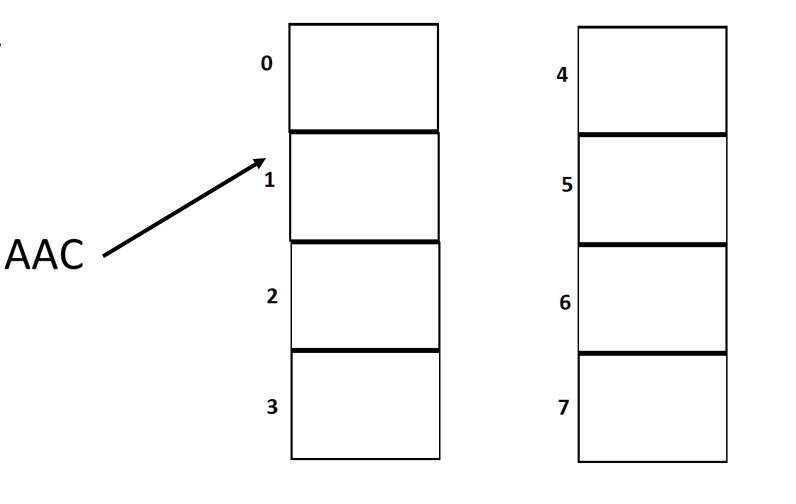
\includegraphics[scale = 0.4]{images/insertion1.png}
  \caption{Odabir lokacije za niz AAC - prikaz po uzoru na [2]}
  \label{fig_insert1}
\end{figure}
Idući na redu je niz ACT. Nakon generiranja sažetaka smješta se u prazni bucket. Budući da je bucket na jednom od dobivenih indeksa već popunjen, sprema se na drugo, prazno mjesto.
\begin{figure}[H]
  \centering
  \setlength{\intextsep}{5pt}
  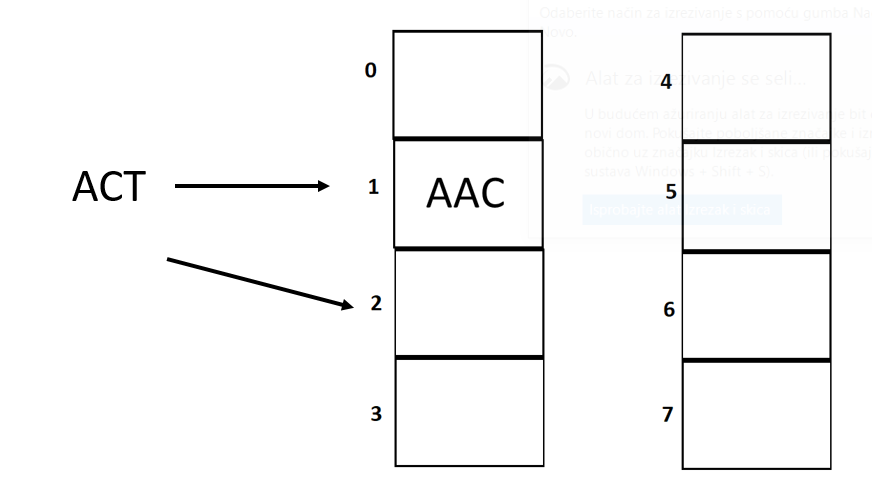
\includegraphics[scale = 0.4]{images/insertion2.png}
  \caption{Odabir lokacije za niz ACT - prikaz po uzoru na [2]}
  \label{fig_insert2}
\end{figure}

Isti korak ponavlja se za niz CTG.
\begin{figure}[H]
  \centering
  \setlength{\intextsep}{5pt}
  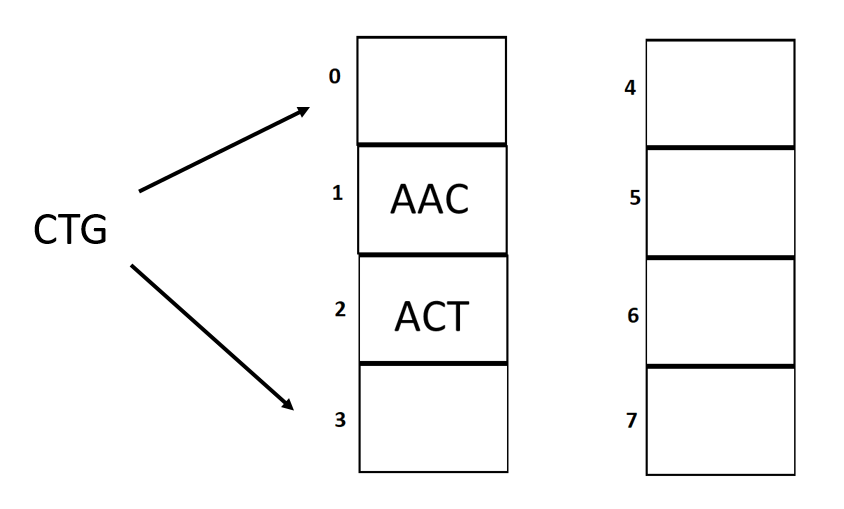
\includegraphics[scale = 0.4]{images/insertion3.png}
  \caption{Odabir lokacije za niz CTG - prikaz po uzoru na [2]}
  \label{fig_insert3}
\end{figure}

Za niz TGA dogodila se situacija da oba pokazivača pokazuju na indekse s već popunjenim bucketima. Tada se u algoritmu događa "izbacivanje". Obabrani se element izbacuje, umeće se TGA, a za izbačeni element traži se nova lokacija. Odabir lokacije razlikuje se od algoritma do algoritma.

\begin{figure}[H]
  \centering
  \setlength{\intextsep}{5pt}
  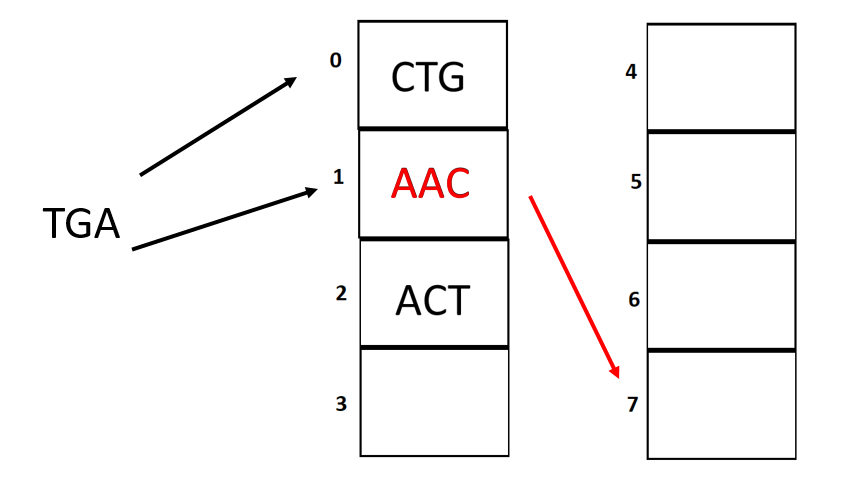
\includegraphics[scale = 0.4]{images/swap1.png}
  \caption{Izbacivanje AAC i ubacivanje TGA - prikaz po uzoru na [2]}
  \label{fig_swap1}
\end{figure}

Za niz GAC također se mora izvršiti izbacivanje starog elementa. 

\begin{figure}[H]
  \centering
  \setlength{\intextsep}{5pt}
  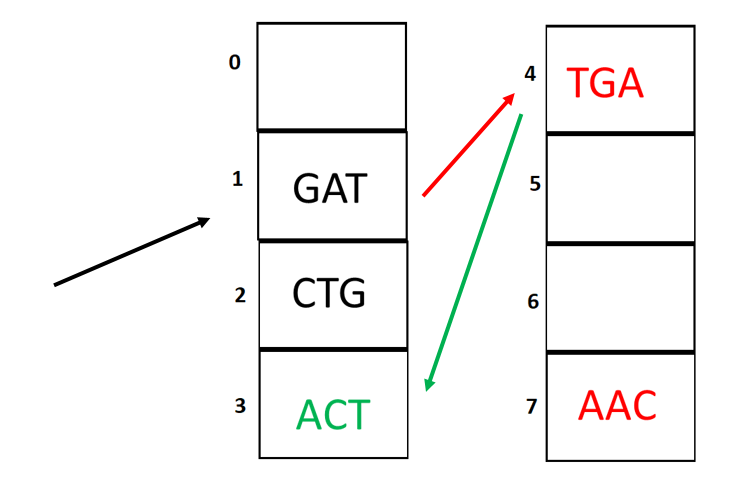
\includegraphics[scale = 0.4]{images/swap2.png}
  \caption{Izbacivanje ACT i ubacivanje GAC - prikaz po uzoru na [2]}
  \label{fig_swap2}
\end{figure}

\begin{figure}[H]
  \centering
  \setlength{\intextsep}{5pt}
  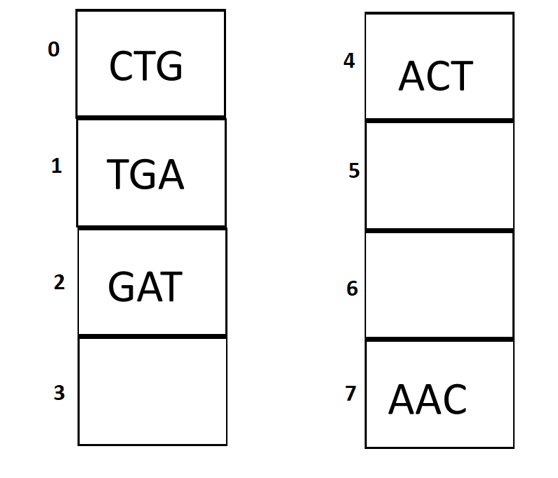
\includegraphics[scale = 0.4]{images/finalalign.png}
  \caption{Konačni razmještaj elemenata - prikaz po uzoru na [2]}
  \label{fig_finalalign}
\end{figure}

Može se primijetiti da što je popunjenost veća, raste i vjerojatnost da će doći do izbacivanja i relokacije starijih elemenata u filteru. Dogodit će se situacije da će element koji se premješta biti premješten na već popunjeni bucket. U tom slučaju prijašnji element će se premjestiti, te će postupak nastaviti sve dok se ne pronađe slobodno mjesto ili se dosegne maksimalan broj operacija premještanja. U slučaju da se dosegne maksimalan broj, to je obično indikator skore popunjenosti filtera. U tom slučaju mogu se poduzeti razne akcije, koje su ponovno različite za svaku implementaciju filtera. \\

TODO NAPOMENA: Eventualno doradit opise, dodat usporedbe tih algoritama iz dokumentacije po čemu se razlikuju, ali neznam dal smijem njihove slike (npr. tablice s vremenskim složenostima i to) jer piše u uputama kao da treba dopuštenje autora. 

 
\chapter{Analiza}

Analiza točnosti, vremena izvođenja i utroška memorije za različite testne slučajeve - ovo nosi 3 boda. Testira se na stvarnim podatcima, kod nas E. coli - rezultati prikazani u tablici ili grafu.

\chapter{Zaključak}
Zaključak.

TODO Komentirati kako naša implementacija radi u odnosu na predloženu, komentirati analizu.

\bibliography{literatura}
\bibliographystyle{fer}

\chapter{Sažetak}
U ovome radu dan je pregled vlastite implementacije rješenja problema opisanog u znanstvenim radovima koja je napravljena u sklopu projekta iz kolegija Bioinformatika 1 na Fakultetu elektrotehnike i računarstva Sveučilišta u Zagrebu. Dan je opis algoritma, motivacija za njegovo korištenje, kao i primjer primjene na odabrani nukleotidni slijed. Nadalje, analiziran je rad algoritma u ovoj implementaciji u odnosu na dosadašnje implementacije, njegove prednosti i nedostatci. \\


\end{document}
